%%%%%%%%%%%%%%%%%%%%%%%%%%%%%%%%%%%%%%%%%
% Wenneker Article
% LaTeX Template
% Version 2.0 (28/2/17)
%
% This template was downloaded from:
% http://www.LaTeXTemplates.com
%
% Authors:
% Vel (vel@LaTeXTemplates.com)
% Frits Wenneker
%
% License:
% CC BY-NC-SA 3.0 (http://creativecommons.org/licenses/by-nc-sa/3.0/)
%
%%%%%%%%%%%%%%%%%%%%%%%%%%%%%%%%%%%%%%%%%

%----------------------------------------------------------------------------------------
%	PACKAGES AND OTHER DOCUMENT CONFIGURATIONS
%----------------------------------------------------------------------------------------

\documentclass[12pt, a4paper, twocolumn]{article} % 10pt font size (11 and 12 also possible), A4 paper (letterpaper for US letter) and two column layout (remove for one column)

\usepackage[utf8]{inputenc}
\usepackage[italian]{babel}

%%%%%%%%%%%%%%%%%%%%%%%%%%%%%%%%%%%%%%%%%
% Wenneker Article
% Structure Specification File
% Version 1.0 (28/2/17)
%
% This file originates from:
% http://www.LaTeXTemplates.com
%
% Authors:
% Frits Wenneker
% Vel (vel@LaTeXTemplates.com)
%
% License:
% CC BY-NC-SA 3.0 (http://creativecommons.org/licenses/by-nc-sa/3.0/)
%
%%%%%%%%%%%%%%%%%%%%%%%%%%%%%%%%%%%%%%%%%

%----------------------------------------------------------------------------------------
%	PACKAGES AND OTHER DOCUMENT CONFIGURATIONS
%----------------------------------------------------------------------------------------

\usepackage[italian]{babel} % English language hyphenation

\usepackage{microtype} % Better typography

\usepackage{amsmath,amsfonts,amsthm} % Math packages for equations

\usepackage[svgnames]{xcolor} % Enabling colors by their 'svgnames'

\usepackage[hang, small, labelfont=bf, up, textfont=it]{caption} % Custom captions under/above tables and figures

\usepackage{booktabs} % Horizontal rules in tables

\usepackage{lastpage} % Used to determine the number of pages in the document (for "Page X of Total")

\usepackage{graphicx} % Required for adding images

\usepackage{enumitem} % Required for customising lists
\setlist{noitemsep} % Remove spacing between bullet/numbered list elements

\usepackage{sectsty} % Enables custom section titles
\allsectionsfont{\usefont{OT1}{phv}{b}{n}} % Change the font of all section commands (Helvetica)

%----------------------------------------------------------------------------------------
%	MARGINS AND SPACING
%----------------------------------------------------------------------------------------

\usepackage{geometry} % Required for adjusting page dimensions

\geometry{
	top=1cm, % Top margin
	bottom=1.5cm, % Bottom margin
	left=2cm, % Left margin
	right=2cm, % Right margin
	includehead, % Include space for a header
	includefoot, % Include space for a footer
	%showframe, % Uncomment to show how the type block is set on the page
}

\setlength{\columnsep}{7mm} % Column separation width

%----------------------------------------------------------------------------------------
%	FONTS
%----------------------------------------------------------------------------------------

\usepackage[T1]{fontenc} % Output font encoding for international characters
\usepackage[utf8]{inputenc} % Required for inputting international characters

\usepackage{XCharter} % Use the XCharter font

%----------------------------------------------------------------------------------------
%	HEADERS AND FOOTERS
%----------------------------------------------------------------------------------------

\usepackage{fancyhdr} % Needed to define custom headers/footers
\pagestyle{fancy} % Enables the custom headers/footers

\renewcommand{\headrulewidth}{0.0pt} % No header rule
\renewcommand{\footrulewidth}{0.4pt} % Thin footer rule

\renewcommand{\sectionmark}[1]{\markboth{#1}{}} % Removes the section number from the header when \leftmark is used

%\nouppercase\leftmark % Add this to one of the lines below if you want a section title in the header/footer

% Headers
\lhead{} % Left header
\chead{\textit{\thetitle}} % Center header - currently printing the article title
\rhead{} % Right header

% Footers
\lfoot{} % Left footer
\cfoot{} % Center footer
\rfoot{\footnotesize Page \thepage\ of \pageref{LastPage}} % Right footer, "Page 1 of 2"

\fancypagestyle{firstpage}{ % Page style for the first page with the title
	\fancyhf{}
	\renewcommand{\footrulewidth}{0pt} % Suppress footer rule
}

%----------------------------------------------------------------------------------------
%	TITLE SECTION
%----------------------------------------------------------------------------------------

\newcommand{\authorstyle}[1]{{\large\usefont{OT1}{phv}{b}{n}\color{DarkRed}#1}} % Authors style (Helvetica)

\newcommand{\institution}[1]{{\footnotesize\usefont{OT1}{phv}{m}{sl}\color{Black}#1}} % Institutions style (Helvetica)

\usepackage{titling} % Allows custom title configuration

\newcommand{\HorRule}{\color{DarkGoldenrod}\rule{\linewidth}{1pt}} % Defines the gold horizontal rule around the title

\pretitle{
	\vspace{-30pt} % Move the entire title section up
	\HorRule\vspace{10pt} % Horizontal rule before the title
	\fontsize{32}{36}\usefont{OT1}{phv}{b}{n}\selectfont % Helvetica
	\color{DarkRed} % Text colour for the title and author(s)
}

\posttitle{\par\vskip 15pt} % Whitespace under the title

\preauthor{} % Anything that will appear before \author is printed

\postauthor{ % Anything that will appear after \author is printed
	\vspace{10pt} % Space before the rule
	\par\HorRule % Horizontal rule after the title
	\vspace{20pt} % Space after the title section
}

%----------------------------------------------------------------------------------------
%	ABSTRACT
%----------------------------------------------------------------------------------------

\usepackage{lettrine} % Package to accentuate the first letter of the text (lettrine)
\usepackage{fix-cm}	% Fixes the height of the lettrine

\newcommand{\initial}[1]{ % Defines the command and style for the lettrine
	\lettrine[lines=3,findent=4pt,nindent=0pt]{% Lettrine takes up 3 lines, the text to the right of it is indented 4pt and further indenting of lines 2+ is stopped
		\color{DarkGoldenrod}% Lettrine colour
		{#1}% The letter
	}{}%
}

\usepackage{xstring} % Required for string manipulation

\newcommand{\lettrineabstract}[1]{
	\StrLeft{#1}{1}[\firstletter] % Capture the first letter of the abstract for the lettrine
	\initial{\firstletter}\textbf{\StrGobbleLeft{#1}{1}} % Print the abstract with the first letter as a lettrine and the rest in bold
}

%----------------------------------------------------------------------------------------
%	BIBLIOGRAPHY
%----------------------------------------------------------------------------------------

% \usepackage[backend=bibtex,style=authoryear,natbib=true]{biblatex} % Use the bibtex backend with the authoryear citation style (which resembles APA)

\addbibresource{example.bib} % The filename of the bibliography

\usepackage[autostyle=true]{csquotes} % Required to generate language-dependent quotes in the bibliography
 % Specifies the document structure and loads requires packages

% \usepackage{textcomp}
%----------------------------------------------------------------------------------------
%	ARTICLE INFORMATION
%----------------------------------------------------------------------------------------

\title{Sound of Data} % The article title

\author{
  \authorstyle{
    % DO NOT TOUCH HSPACEs!! @Momo
    Riccardo Cervero \hspace{25pt} 794126 \\  % x + 4
    Marco Ferrario \hspace{44pt}  795203 \\   % x + 23
    Pranav Kasela \hspace{46.5pt} 846965 \\   % x + 25.5
    Federico Moiraghi \hspace{21pt} 799735    % x
  } % Authors
  \newline\newline
  \institution{Università degli Studi di Milano Bicocca}
}

\date{Anno Accademico 2018/19} % Add a date here if you would like one to appear underneath the title block, use \today for the current date, leave empty for no date

%----------------------------------------------------------------------------------------

\begin{document}

\maketitle % Print the title

\thispagestyle{firstpage} % Apply the page style for the first page (no headers and footers)

%----------------------------------------------------------------------------------------
%	ABSTRACT
%----------------------------------------------------------------------------------------

\lettrineabstract{Obiettivo del progetto è analizzare la discussione mediatica riguardante i soggetti del mondo musicale contemporaneo e passato, ottenendo, grazie alla gestione in tempo reale di un flusso di tweets, gli artisti, le produzioni e i generi citati all'interno del testo, in modo da produrre uno schema a grafo in grado di rappresentare efficacemente la composizione dei topic musicali nell'arco del tempo, e osservare quali legami possano esistere fra le comunità formate da utenti che scrivono degli stessi argomenti.}
\hfill

\tableofcontents
\hfill
\newpage

%----------------------------------------------------------------------------------------
%	ARTICLE CONTENTS
%----------------------------------------------------------------------------------------
\part{Introduzione}
I traguardi posti dal progetto \textit{Sound of Data}\footnote{\url{https://github.com/pkasela/Sound-of-Data}}, hanno innanzitutto richiesto la raccolta di un volume di dati sufficienti per costruire un \textit{knowledge graph} adeguato alla materia. Scaricato un \textit{dump} di \url{musicbrainz.org} come database relazionale - già esportato in formato \textit{Tabular Separated Values} dai manutentori-, si è provveduto ad importarlo all'interno di Apache Hadoop\footnote{\url{https://hadoop.apache.org}} per effettuare una rapida pulizia preliminare, e infine esportarlo, in modo tale da costruire un grafo Neo4J\footnote{\url{https://neo4j.com}}.
Costituita quindi la base di conoscenza su cui operare, i \textit{tweet} sono stati raccolti in tempo reale grazie ad Apache Kafka\footnote{\url{https://kafka.apache.org}}. Durante questa fase di \textit{streaming}, essi subiscono varie operazioni di \textit{preparation} e vengono filtrati da un rudimentale strumento di \textit{instance matching}. Grazie ad un efficiente plug-in che permette all'utente di sfruttare il \textit{DBMS Neo4j} identicamente a qualsiasi \textit{Consumer} di \textit{Apache Kafka}, il risultato si costituisce automaticamente in uno schema a grafo. Dopo la complessa fase di gestione e raccolta dei dati, è stato possibile condurre un'analisi finale sulle dinamiche della discussione musicale instauratesi fra i singoli utenti all'interno di comunità astratte ed estremamente mutevoli, e sulle relazioni, più o meno intense, esistenti fra di esse. Le progressiva composizione che i nodi associati ai tweet assumono all'interno del grafo viene studiata ad intervalli regolari, corrispondenti alle quattro fasce orarie relative al mattino, pomeriggio, sera, notte. Si è preferito adoperare tale ciclo giornaliero, anzichè un più ampio ciclo settimanale, o addirittura mensile, per due ragioni precise. Innanzitutto, esso si rivela migliore dal punto di vista interpretativo: risulta di estremo interesse osservare i trend ricorrenti nei vari momenti della giornata, piuttosto che rifersi all'arco settimanale. Inoltre, il ciclo giornaliero ha il vantaggio di non risentire della distorsione provocata dagli eventi, siano essi previsti o imprevisti. Infatti, essendo in grado di assorbire l'interesse della gran parte dell'opinione pubblica per interi giorni e settimane, questi penalizzano l'analisi e concentrano tutti gli utenti verso un numero limitato di argomenti musicali.\ 
Due esempi riguardanti tale problematica, e le sue conseguenze negative, possono essere citati per quanto concerne il genere \textit{"drone"}. Durante il periodo di raccolta, si sono succeduti due eventi particolarmente rilevanti. Il primo coincide con l'abbattimento di un drone americano, causa di nuove tensioni fra Stati Uniti e Iran\footnote{\url{http://www.ansa.it/sito/notizie/mondo/mediooriente/2019/06/20/iran-pasdaran-abbattuto-drone-usa_b8922ea0-e61c-436b-8f66-60f3be32ed21.html}}, mentre il secondo consiste in uno spettacolo di droni luminosi a Torino\footnote{\url{https://www.guidatorino.com/eventi-torino/san-giovanni-torino-droni-2019/}}. Raccogliendo la preoccupazione o l'interesse di centinaia di utenti, essi hanno fatto sì che il cluster del genere \textit{"drone"}, la cui parola presenta inoltre un evidente difetto di polisemia, fosse sproporzionato rispetto alle dimensioni delle altre comunità, se osservato nella settimana e nei giorni in corrispondenza dei due avvenimenti. Tuttavia, se vista su un arco giornaliero, questa distorsione non risulta eccessivamente grave. Per evitare che altri eventi, seppur riferiti effettivamente al mondo della musica, potessero nuocere alla bontà dello studio, si è pertanto deciso di adoperare queste quattro fasce orarie come intervalli temporali di riferimento.

\hfill
\newpage
\part{Costruzione dello \textit{knowledge graph}}

\section{Data Cleaning con Python e Pig}
%Riferimenti `Bibliografici'
%https://www.infoq.com/articles/apache-tez-saha-murthy/
%https://tez.apache.org/


I dati vengono scaricati dal sito di musicbrainz attraverso il file \textit{get\_data.py}\footnote{\url{https://github.com/pkasela/Sound-of-Data/blob/master/musicbrainz_data/Data_Cleaning/get_data.py}}, e, sempre al suo interno, gestiti preliminarmente, in modo da sostituire, attraverso il comando sed, tutti i caratteri "\\N" con campi vuoti in tutti i file, e salvare solamente i file necessari alla creazione del \textit{database} a grafo. 
La lista dei generi è anch'essa presente sul sito di \textit{musicbrainz}. Pertanto, questa viene estratta e salvata all'interno del codice attraverso uno scraper. Poi, grazie al confronto con il file \textit{tag}, vengono individuati e rimossi tutti i \textit{tag} che non rappresentano un genere musicale.

%%%%%%
%%%%%%%%%%%
%%%%%%%%%%%%%%%%
%%%% Ma lo schema iniziale va messo?
%%%% Io dico di no al massimo lo schema finale
%%%%%%%%%%%%%%%%
%%%%%%%%%%%
%%%%%%

I file vengono successivamente trasferiti e processati all'interno del \textit{file system} HDFS. Nel dettaglio, questa fase viene eseguita attraverso l'utilizzo di Apache Pig, una piattaforma atta proprio all'elaborazione dei dati. La decisione di utilizzare Pig anzichè SQL dipende principalmente dal fatto che il caricamento dei dati in un database relazionale sia molto più lenta, e dalla capacità di Pig di riuscire a sfruttare a pieno la potenza di HDFS.
L'\textit{engine} adoperato in combinazione con Pig è Tez, che rende molto più veloce il \textit{processing} dei dati, saltando diverse fasi di scrittura dei risultati parziali su HDFS.
Apache Tez è costruito direttamente sopra YARN, e migliora drasticamente la velocità rispetto a \textit{MapReduce}, mantenendo la sua stessa scalabilità [Figura 1]. 

\begin{figure*}
	\centering
	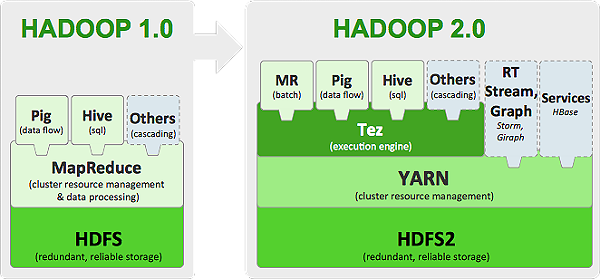
\includegraphics{hadoop2.png}
	\caption{Differenza archittetura di HADOOP 1.0 con MR e 2.0 con Tez}
\end{figure*}

Più precisamente, la velocità di esecuzione è ottenuta grazie all'invio diretto dei dati da un processo all'altro, evitando la scrittura all'interno del file system, eccezion fatta per i checkpoints. Inoltre, la definizione del \textit{job} sfrutta i \textit{Directed Acyclic Graph}, dove i vertici rappresentano gli step del processo e gli archi la connessione tra i vertici \textit{Producer} e \textit{Consumer} [Figura 2].

\begin{figure*}
	\centering
	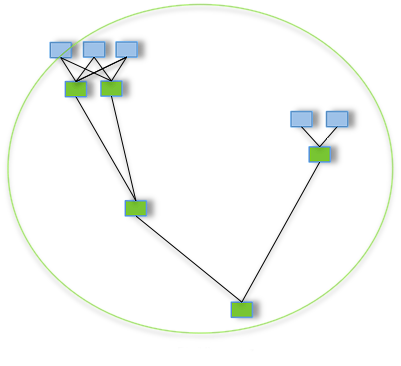
\includegraphics{tez.png}
	\caption{Archittetura di HADOOP 2.0 con Tez}
\end{figure*}

Conclusa la fase di pulizia, i dati vengono trasferiti all'esterno di HDFS, sul filesystem, e i risultati di Pig sono uniti mediante il comando \textit{cat} di \textit{Linux}. 
A questo punto i dati sono pronti per essere importati in Neo4j.

%%%%%%
%%%%%%%%%%%
%%%%%%%%%%%%%%%%
%%%% Conviene mettere lo schema finale delle tabelle (dopo lo metto)
%%%%%%%%%%%%%%%%
%%%%%%%%%%%
%%%%%%

\section{Import dei dati in Neo4J}
%Reference
%https://neo4j.com/docs/operations-manual/current/tutorial/import-tool/

Infine, il risultato dell'elaborazione svolta da Pig viene caricato all'interno del \textit{DBMS Neo4j}, usando neo4j-import, aggiungendo degli indici sui \textit{gid} delle varie entità, in modo da velocizzare la ricerca da svolgere successivamente.
%cosa altro si deve scrivere hahaha

\hfill
\newpage
\part{Analisi dei tweet}
\section{Elaborazione mediante Apache Kafka}
%Reference 
%https://github.com/neo4j-contrib/neo4j-streams
%https://riak-python-client.readthedocs.io/en/1.5-stable/tutorial.html
Nella fase di analisi in tempo reale, i tweet vengono filtrati ed elaborati mediante una sequenza di operazioni, attraverso una \textit{pipeline} costituita dalla concatenazione di due coppie di processi Producer e Consumer. L'architettura di elaborazione in \textit{streaming} è stata configurata in questa maniera affinchè garantisse una maggiore scalabilità ed una migliore performance, riuscendo a reggere più alti volumi di \textit{tweet} in ingresso.\ 
Questi vengono estratti grazie all'API \textit{Tweepy}\footnote{\url{https://tweepy.readthedocs.io/en/latest/}} per Python - utilizzando come parole chiave di ricerca 400 generi musicali fra i 419 ottenuti dallo scraping della pagina \textit{'https://musicbrainz.org/genres'}, e filtrando soltanto i testi pubblicati in lingua italiana - e inviati ad una prima Topic come messaggi di un \textit{Producer} di Kafka, inizializzato mediante la libreria \textit{Kafka-python}\footnote{\url{https://pypi.org/project/kafka-python/}}. 
All'interno di un secondo file\footnote{\url{https://github.com/pkasela/Sound-of-Data/blob/master/NL/Kafka_Producer_2.py}}, associato ad un nuovo processo Producer, dunque ad una seconda Topic connessa in \textit{streaming} con la precedente, il JSON grezzo che costituisce ciascun \textit{tweet} in ingresso viene processato in vari step dalla funzione \textit{tweet\_preparations}. La prima fase coincide con l'estrazione dello \textit{"screen name"} dell'utente, del contenuto postato e dell'ora e data precisa di pubblicazione. 
In particolare, il testo viene modificato in modo da rendere leggibili i caratteri speciali e i cosiddetti \textit{escape characters}. 
La seconda fase sfrutta l'API di \textit{Botometer}\footnote{\url{https://rapidapi.com/OSoMe/api/botometer/details}} per calcolare la probabilità - definita \textit{"score"} - che un profilo sia in realtà gestito da un BOT, osservandone il comportamento passato.
Poiché questo tipo di gestione automatizzata degli account altera, spesso fortemente, la discussione mediatica, aumentando arbitrariamente il flusso di determinati contenuti, si è deciso di non archiviare i \textit{tweet} appartenenti a tali profili. 
Nel dettaglio, se lo score associato all'utente di ogni \textit{tweet} supera una soglia fissata al 90\%, lo \textit{screen name} viene memorizzato all'interno di una \textit{blacklist}, altrimenti smistato in una \textit{whitelist}, in modo che il programma possa riconoscere più velocemente ogni profilo ed evitare inutili ricalcoli. 
Per aumentare l'efficienza di questo \textit{storage} e garantire la scalabilità, si è scelto di adoperare il \textit{data store Riak}, di tipo \textit{NoSQL Key-Value}, attraverso la propria libreria in Python\footnote{\url{https://github.com/basho/riak-python-client}}. 
La terza fase verifica che il testo sia effettivamente legato al tema musicale. 
La quarta e ultima fase consiste nel riconoscimento delle parole riguardanti il contesto musicale, aggiungendo al dizionario prodotto dalle fasi precedenti tre chiavi corrispondenti rispettivamente alla lista di artisti, album o canzoni estratti dal testo analizzato. 
Questi due step sono permessi dall'uso dell'API fornita dal sito \textit{musicbrainz.org}. 
Per maggiori dettagli sul processo di analisi semantica, si rimanda alla sezione dedicata. 
Infine, ogniqualvolta si verificano le due condizioni note, cioè che l'utente non abbia probabilità elevata di essere un BOT e che il testo pubblicato si riferisca effettivamente al mondo della musica, ciascun risultato della funzione \textit{tweet\_preparations} viene ricodificato e passato come messaggio al secondo \textit{Producer} di \textit{Apache Kafka} - menzionato in precedenza-, che effettuerà l'invio del dato finale alla \textit{topic} nominata \textit{"KafkaTopic"}. 
Grazie all'utilizzo di questa piattaforma, il flusso di \textit{feed} viene gestito in tempo reale, assicurando bassissima latenza e grande scalabilità. 

\section{Consuming dei Tweets in Neo4j}
Un principale vantaggio di \textit{Apache Kafka} consiste nella capacità di connettersi efficientemente a sistemi esterni, garantendo in tal modo la continuità dello \textit{stream} di dati da una fonte - la class \textit{Listener} adoperata in Python per "ascoltare" i tweet grazie all'API Tweepy -, ad una \textit{"landing zone"}, che in questo caso corrisponde al DBMS \textit{Neo4j}. 
Si è scelto di effettuare lo \textit{storage} dei tweets in un \textit{GraphDB}, e in particolare \textit{Neo4j}, tra le varie motivazioni, per le sue caratteristiche di estrema scalabilità, efficienza nella gestione, elevata capacità di adattamento al fenomeno di studio e interpretabilità dei dati.
L'esportazione diretta dei tweets da \textit{Apache Kafka} all'interno del \textit{data store} avviene grazie al \textit{plug-in} di \textit{Neo4j} chiamato \textit{"Neo4j Streams Consumer"}. Questo si configura come un'applicazione che effettua un'ingestione diretta e automatizzata all'interno di \textit{Neo4j}, permettendo la lettura dei dati presenti nella \textit{topic} identicamente a qualsiasi applicazione \textit{Consumer} di \textit{Kafka}. 
\textit{Neo4j Streams Consumer} permette all'utente di specificare arbitrariamente le relazioni, entità e proprietà in cui i \textit{payloads} di \textit{Apache Kafka}, corrispondenti al JSON di ciascun tweet importato, dovranno essere organizzati per costruire progressivamente il grafo.
La struttura di quest'ultimo viene dichiarata attraverso un \textit{Cypher template}, ovvero un insieme di \textit{queries} semantiche di \textit{Cypher}, all'interno di un file di configurazione, che nel caso presentato è il \textit{"docker-compose.yml"}\footnote{\url{https://github.com/pkasela/Sound-of-Data/blob/master/Neo4j\%20\%26\%20kafka/docker-compose\%20configuration.yml}}, poiché il progetto viene eseguito mediante \textit{Docker Desktop}, in quanto quest'ultimo presenta il vantaggio di riuscire a far comunicare automaticamente e in maniera trasparente i containers coinvolti. 
Una volta specificato il \textit{Cypher template}, installato il \textit{plugin} all'interno del \textit{Docker}, e successivamente montati i container e i relativi collegamenti, la fase di mera esecuzione del progetto avviene mediante la funzione denominata \textit{"streams.consume"}, la quale crea immediatamente la struttura del grafo come indicato. 
Nello specifico, all'arrivo di un \textit{tweet} verranno dunque aggiunti i nodi \textit{"Tweet"},\textit{"User"} ed un terzo che riporterà ora e data di pubblicazione. 
Il primo conterrà le \textit{property keys} del testo \textit{"text"}, e dello \textit{"screen\_name"}. 
Il secondo, invece, conterrà solamente la proprietà \textit{"name"}, che riporta lo \textit{screen name}. 
Tra primi i due nuovi nodi verrà generata la relazione \textit{"BELONGS\_TO"}, ad indicare il profilo di appartenenza di ciascun post, mentre "User" sarà connesso all'ora/data di pubblicazione da un \textit{edge} etichettato come \textit{"Twitted"}.
In più, il programma effettuerà automaticamente una \textit{merge} della coppia appena generata con i nodi già presenti all'interno del grafo, importati precedentemente da \textit{musicbrainz.org}, nella seguente maniera: quando il testo cita, ad esempio, un artista, il software crea la relazione \textit{"TALKS\_ABOUT",} rappresentata da un arco connesso al nodo a cui appartiene il \textit{"value"} di quel preciso artista - cioè il suo id -, il quale sarà già a sua volta collegato ai generi musicali cui appartengono le proprie produzioni. In questo modo, il nodo riferito al genere costituirà il centro di ogni cluster di utenti. 
Lo stesso accade per quanto riguarda le \textit{labels} relative al titolo di una canzone, oppure di un album. 
A questo punto, il grafo apparirà direttamente cosparso di nodi utente, raggruppati in comunità a seconda dell'oggetto dei propri \textit{tweet}, ingrandendosi e variando in base alle dinamiche interne alla discussione mediatica nell'arco di vari cicli orari e giornalieri. 
Grazie a questa semplice struttura, l'analisi avviene già in maniera grafica e trasparente, e l'utente è in grado di distinguere la grandezza di queste comunità variabili, intendere quali legami esistano fra di esse, e quanto questi siano intensi.
Per ottenere queste informazioni, è infatti sufficiente scaricare un \textit{dump} del grafo a intervalli regolari e confrontare i vari risultati. 
Il risultato finale, dall'interfaccia web di \texti{Neo4j}, apparirà come nella Figura 3. \\
\\
Invece, la composizione dei cluster, delle comunità ben separate, verrà mostrata come nella Figura 4.

\begin{figure*}
	\centering
	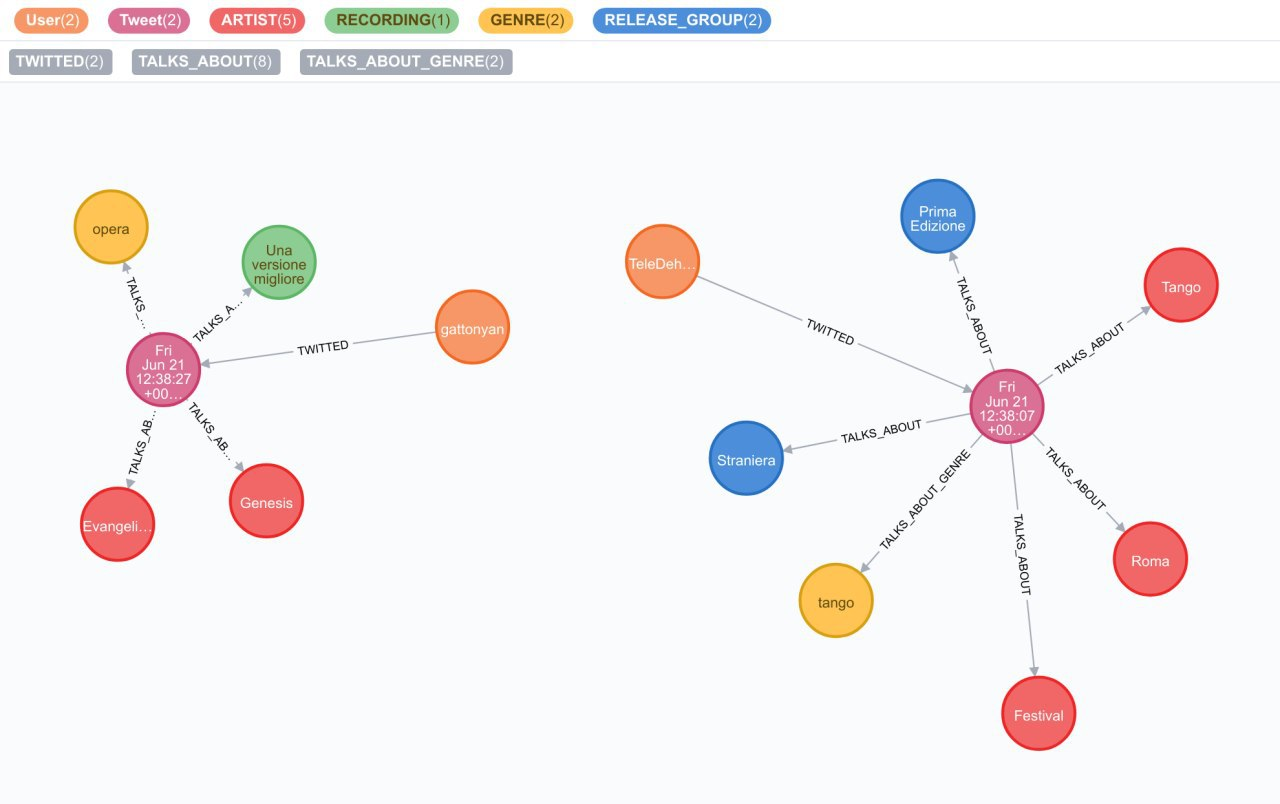
\includegraphics{small_graph.png}
	\caption{Configurazione della struttura del grafo}
\end{figure*}

\begin{figure*}
	\centering
	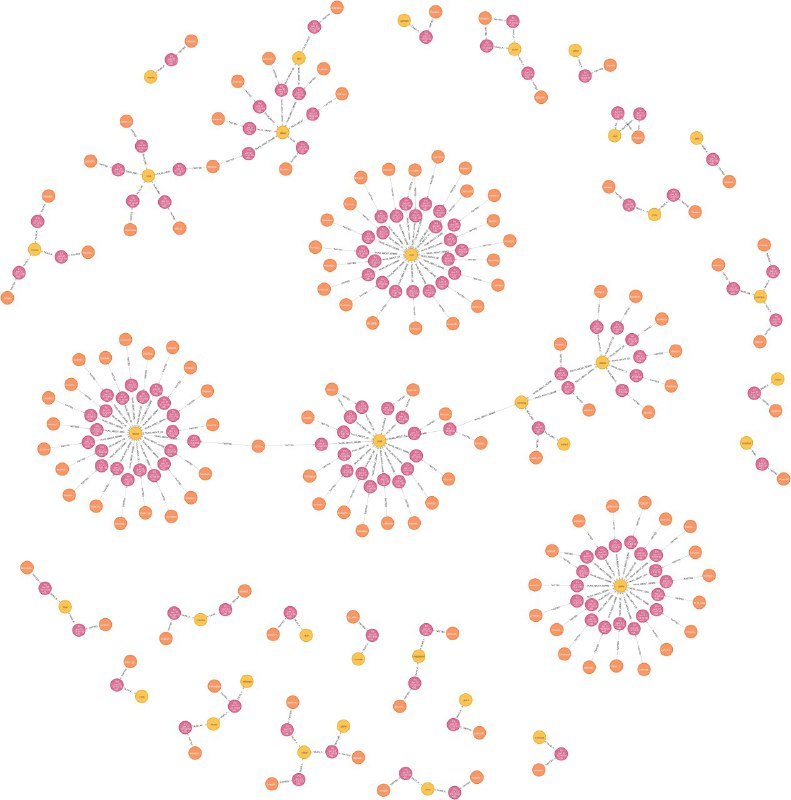
\includegraphics{big_graph.png}
	\caption{Composizione parziale delle comunità all'interno del grafo}
\end{figure*}

\section{Riconoscimento delle istanze nel testo}
Data la mole di dati scaricabili, si è deciso di costruire un strumento di \textit{instance matching} creato \textit{ad hoc} per i tweet.
Vista la scarsa abilità degli algoritmi basati su reti neurali e \textit{deep learning} nell'analisi del breve (e quindi decontestualizzato) testo di un tweet, si è costruito un modello per l'identificazione di ipotetiche entità su cui basarsi per confronti col database, sfruttando i \textit{gid}, i codici identificativi di musicbrainz disponibile grazie all'API\footnote{\url{https://python-musicbrainzngs.readthedocs.io/en/v0.6/}} offerta da \url{musicbrainz.org} stesso).

\subsection{Identificazione delle entità}
Le entità sono riconosciute non mediante \textit{machine learning} ma grazie a semplici stratagemmi linguistici.
Prima di tutto il testo del tweet è ripulito da eventuali abbreviazioni gergali; subito dopo sono ricercate le parole nel testo che non risultano essere italiane: analizzando tweet in lingua italiana, si presume che una stringa in lingua diversa abbia una certa importanza.
Per fare questo è usato un mero correttore ortografico che evidenzia quali parole non sono riconosciute; di aiuto nel compito è anche una semplice espressione regolare che tenta di stabilire quali parole non seguano la costruzione sillabica italiana (rientrando quindi o nella categoria dei sostantivi della quinta classe o, nei casi fortunati, nelle entità cercate): secondo le regole linguistiche, una sillaba correttamente formata è composta da un numero massimo di tre consonanti seguita da una vocale e da al più una sola consonante - o vocale con suono consonantico, formando quindi un dittongo.
Alle entità così individuate si aggiungono tutte le parole scritte in maiuscolo - che in un testo di così bassa formalità non sempre coincidono coi nomi propri-, anche se a inizio frase.
Grazie all'uso della punteggiatura - le virgolette - e delle preposizioni, si tenta inoltre di stabilire se l'entità rilevata è un presunto autore o una presunta opera.
Per individuare gli id delle entità riconosciute con il metodo descritto precedentemente, è stato utilizzato Python con la libreria \textit{Musicbrainzngs}.
Attraverso le funzioni \textit{search} è possibile consultare il database sfruttando un server di ricerca costruito utilizzando la tecnologia \text{Lucene}.
\textit{Musicbrainz} è interrogato con la funzione search\_artists per le entità riconosciute come autori, search\_recordings per quelle individuate come canzoni, ed entrambe, con in aggiunta search\_release\_groups (funzione relativa alla ricerca degli album), per quelle la cui tipologia è incerta.
La problematica principale emersa in questa parte è stata la difficoltà ad attribuire all’entità analizzata l’id che la caratterizza effettivamente.
Sono infatti molto frequenti i casi di omonimia tra canzoni ed album relativi ad artisti differenti ed è quindi possibile che il risultato ottenuto non sia quello desiderato.
Per cercare di aumentare le probabilità di restituire i \textit{gid} corretti è stato impostato un valore di similarità pari a 0.95 nell’interrogazione al database. Inoltre per le canzoni e per gli album si è provveduto a verificare la presenza di corrispondenze con le entità artisti precedentemente individuate nel testo.

\subsection{Prestazioni del modello e margini di miglioramento}
Nonostante il modello semantico offra una buona \textit{performance} nella selezione dei testi riferiti al mondo musicale e nel riconoscimento delle istanze nel testo, continua a presentare alcune imperfezioni. Un primo difetto deriva dalla difficoltà nella gestione dei casi polisemici: i generi nominati \textit{"drone"}, \textit{"dance"}, \textit{"club"} e "opera" risultano, ovviamente, estremamente complessi da interpretare per uno strumento rudimentale, incapace di distinguere perfettamente il contesto all'interno del quale queste parole vengono utilizzate. Più nel dettaglio: il termine "club" viene più spesso citato all'interno di testi riguardanti qualsiasi tipo di associazione; la parola "drone", come già spiegato nell'introduzione, indica, nella maggior parte dei casi, l'aeromobile; "opera" possiede numerosi significati, oltre al genere musicale; l'espressione "dance" è frequentemente slegata alla musica. \\
Una seconda problematica è sorta dopo aver rilevato alcuni \textit{tweet} in lingua straniera che citavano il termine \textit{trap} senza riferirsi al genere musicale, successivamente rimossi.\\
Pertanto, il modello raggiunge buoni risultati nell'ambito di tale progetto, rendendo comunque necessari ulteriori tentativi di miglioramento della sua capacità di riconoscere il contesto all'interno del quale le parole vengono citate.

\hfill
\newpage
\part{Visualizzazioni dei dati}

\hfill
\newpage
\part{Risultati e conclusioni}
Quanti tweet abbiamo raccolto? Cosa abbiamo osservato? Quali dinamiche esistono tra le comunità e quali sono quelle più grandi?


%----------------------------------------------------------------------------------------
%	BIBLIOGRAPHY
%----------------------------------------------------------------------------------------

\hfill
\newpage
\printbibliography[title={Bibliografia e sitografia}]

%----------------------------------------------------------------------------------------

\end{document}
